% Options for packages loaded elsewhere
\PassOptionsToPackage{unicode}{hyperref}
\PassOptionsToPackage{hyphens}{url}
\PassOptionsToPackage{dvipsnames,svgnames,x11names}{xcolor}
%
\documentclass[
  letterpaper,
  DIV=11,
  numbers=noendperiod]{scrartcl}

\usepackage{amsmath,amssymb}
\usepackage{iftex}
\ifPDFTeX
  \usepackage[T1]{fontenc}
  \usepackage[utf8]{inputenc}
  \usepackage{textcomp} % provide euro and other symbols
\else % if luatex or xetex
  \usepackage{unicode-math}
  \defaultfontfeatures{Scale=MatchLowercase}
  \defaultfontfeatures[\rmfamily]{Ligatures=TeX,Scale=1}
\fi
\usepackage{lmodern}
\ifPDFTeX\else  
    % xetex/luatex font selection
\fi
% Use upquote if available, for straight quotes in verbatim environments
\IfFileExists{upquote.sty}{\usepackage{upquote}}{}
\IfFileExists{microtype.sty}{% use microtype if available
  \usepackage[]{microtype}
  \UseMicrotypeSet[protrusion]{basicmath} % disable protrusion for tt fonts
}{}
\makeatletter
\@ifundefined{KOMAClassName}{% if non-KOMA class
  \IfFileExists{parskip.sty}{%
    \usepackage{parskip}
  }{% else
    \setlength{\parindent}{0pt}
    \setlength{\parskip}{6pt plus 2pt minus 1pt}}
}{% if KOMA class
  \KOMAoptions{parskip=half}}
\makeatother
\usepackage{xcolor}
\ifLuaTeX
  \usepackage{luacolor}
  \usepackage[soul]{lua-ul}
\else
  \usepackage{soul}
  
\fi
\setlength{\emergencystretch}{3em} % prevent overfull lines
\setcounter{secnumdepth}{-\maxdimen} % remove section numbering
% Make \paragraph and \subparagraph free-standing
\ifx\paragraph\undefined\else
  \let\oldparagraph\paragraph
  \renewcommand{\paragraph}[1]{\oldparagraph{#1}\mbox{}}
\fi
\ifx\subparagraph\undefined\else
  \let\oldsubparagraph\subparagraph
  \renewcommand{\subparagraph}[1]{\oldsubparagraph{#1}\mbox{}}
\fi

\usepackage{color}
\usepackage{fancyvrb}
\newcommand{\VerbBar}{|}
\newcommand{\VERB}{\Verb[commandchars=\\\{\}]}
\DefineVerbatimEnvironment{Highlighting}{Verbatim}{commandchars=\\\{\}}
% Add ',fontsize=\small' for more characters per line
\usepackage{framed}
\definecolor{shadecolor}{RGB}{241,243,245}
\newenvironment{Shaded}{\begin{snugshade}}{\end{snugshade}}
\newcommand{\AlertTok}[1]{\textcolor[rgb]{0.68,0.00,0.00}{#1}}
\newcommand{\AnnotationTok}[1]{\textcolor[rgb]{0.37,0.37,0.37}{#1}}
\newcommand{\AttributeTok}[1]{\textcolor[rgb]{0.40,0.45,0.13}{#1}}
\newcommand{\BaseNTok}[1]{\textcolor[rgb]{0.68,0.00,0.00}{#1}}
\newcommand{\BuiltInTok}[1]{\textcolor[rgb]{0.00,0.23,0.31}{#1}}
\newcommand{\CharTok}[1]{\textcolor[rgb]{0.13,0.47,0.30}{#1}}
\newcommand{\CommentTok}[1]{\textcolor[rgb]{0.37,0.37,0.37}{#1}}
\newcommand{\CommentVarTok}[1]{\textcolor[rgb]{0.37,0.37,0.37}{\textit{#1}}}
\newcommand{\ConstantTok}[1]{\textcolor[rgb]{0.56,0.35,0.01}{#1}}
\newcommand{\ControlFlowTok}[1]{\textcolor[rgb]{0.00,0.23,0.31}{#1}}
\newcommand{\DataTypeTok}[1]{\textcolor[rgb]{0.68,0.00,0.00}{#1}}
\newcommand{\DecValTok}[1]{\textcolor[rgb]{0.68,0.00,0.00}{#1}}
\newcommand{\DocumentationTok}[1]{\textcolor[rgb]{0.37,0.37,0.37}{\textit{#1}}}
\newcommand{\ErrorTok}[1]{\textcolor[rgb]{0.68,0.00,0.00}{#1}}
\newcommand{\ExtensionTok}[1]{\textcolor[rgb]{0.00,0.23,0.31}{#1}}
\newcommand{\FloatTok}[1]{\textcolor[rgb]{0.68,0.00,0.00}{#1}}
\newcommand{\FunctionTok}[1]{\textcolor[rgb]{0.28,0.35,0.67}{#1}}
\newcommand{\ImportTok}[1]{\textcolor[rgb]{0.00,0.46,0.62}{#1}}
\newcommand{\InformationTok}[1]{\textcolor[rgb]{0.37,0.37,0.37}{#1}}
\newcommand{\KeywordTok}[1]{\textcolor[rgb]{0.00,0.23,0.31}{#1}}
\newcommand{\NormalTok}[1]{\textcolor[rgb]{0.00,0.23,0.31}{#1}}
\newcommand{\OperatorTok}[1]{\textcolor[rgb]{0.37,0.37,0.37}{#1}}
\newcommand{\OtherTok}[1]{\textcolor[rgb]{0.00,0.23,0.31}{#1}}
\newcommand{\PreprocessorTok}[1]{\textcolor[rgb]{0.68,0.00,0.00}{#1}}
\newcommand{\RegionMarkerTok}[1]{\textcolor[rgb]{0.00,0.23,0.31}{#1}}
\newcommand{\SpecialCharTok}[1]{\textcolor[rgb]{0.37,0.37,0.37}{#1}}
\newcommand{\SpecialStringTok}[1]{\textcolor[rgb]{0.13,0.47,0.30}{#1}}
\newcommand{\StringTok}[1]{\textcolor[rgb]{0.13,0.47,0.30}{#1}}
\newcommand{\VariableTok}[1]{\textcolor[rgb]{0.07,0.07,0.07}{#1}}
\newcommand{\VerbatimStringTok}[1]{\textcolor[rgb]{0.13,0.47,0.30}{#1}}
\newcommand{\WarningTok}[1]{\textcolor[rgb]{0.37,0.37,0.37}{\textit{#1}}}

\providecommand{\tightlist}{%
  \setlength{\itemsep}{0pt}\setlength{\parskip}{0pt}}\usepackage{longtable,booktabs,array}
\usepackage{calc} % for calculating minipage widths
% Correct order of tables after \paragraph or \subparagraph
\usepackage{etoolbox}
\makeatletter
\patchcmd\longtable{\par}{\if@noskipsec\mbox{}\fi\par}{}{}
\makeatother
% Allow footnotes in longtable head/foot
\IfFileExists{footnotehyper.sty}{\usepackage{footnotehyper}}{\usepackage{footnote}}
\makesavenoteenv{longtable}
\usepackage{graphicx}
\makeatletter
\def\maxwidth{\ifdim\Gin@nat@width>\linewidth\linewidth\else\Gin@nat@width\fi}
\def\maxheight{\ifdim\Gin@nat@height>\textheight\textheight\else\Gin@nat@height\fi}
\makeatother
% Scale images if necessary, so that they will not overflow the page
% margins by default, and it is still possible to overwrite the defaults
% using explicit options in \includegraphics[width, height, ...]{}
\setkeys{Gin}{width=\maxwidth,height=\maxheight,keepaspectratio}
% Set default figure placement to htbp
\makeatletter
\def\fps@figure{htbp}
\makeatother
% definitions for citeproc citations
\NewDocumentCommand\citeproctext{}{}
\NewDocumentCommand\citeproc{mm}{%
  \begingroup\def\citeproctext{#2}\cite{#1}\endgroup}
\makeatletter
 % allow citations to break across lines
 \let\@cite@ofmt\@firstofone
 % avoid brackets around text for \cite:
 \def\@biblabel#1{}
 \def\@cite#1#2{{#1\if@tempswa , #2\fi}}
\makeatother
\newlength{\cslhangindent}
\setlength{\cslhangindent}{1.5em}
\newlength{\csllabelwidth}
\setlength{\csllabelwidth}{3em}
\newenvironment{CSLReferences}[2] % #1 hanging-indent, #2 entry-spacing
 {\begin{list}{}{%
  \setlength{\itemindent}{0pt}
  \setlength{\leftmargin}{0pt}
  \setlength{\parsep}{0pt}
  % turn on hanging indent if param 1 is 1
  \ifodd #1
   \setlength{\leftmargin}{\cslhangindent}
   \setlength{\itemindent}{-1\cslhangindent}
  \fi
  % set entry spacing
  \setlength{\itemsep}{#2\baselineskip}}}
 {\end{list}}
\usepackage{calc}
\newcommand{\CSLBlock}[1]{\hfill\break\parbox[t]{\linewidth}{\strut\ignorespaces#1\strut}}
\newcommand{\CSLLeftMargin}[1]{\parbox[t]{\csllabelwidth}{\strut#1\strut}}
\newcommand{\CSLRightInline}[1]{\parbox[t]{\linewidth - \csllabelwidth}{\strut#1\strut}}
\newcommand{\CSLIndent}[1]{\hspace{\cslhangindent}#1}

\KOMAoption{captions}{tableheading}
\makeatletter
\@ifpackageloaded{caption}{}{\usepackage{caption}}
\AtBeginDocument{%
\ifdefined\contentsname
  \renewcommand*\contentsname{Índice}
\else
  \newcommand\contentsname{Índice}
\fi
\ifdefined\listfigurename
  \renewcommand*\listfigurename{Lista de Figuras}
\else
  \newcommand\listfigurename{Lista de Figuras}
\fi
\ifdefined\listtablename
  \renewcommand*\listtablename{Lista de Tabelas}
\else
  \newcommand\listtablename{Lista de Tabelas}
\fi
\ifdefined\figurename
  \renewcommand*\figurename{Figura}
\else
  \newcommand\figurename{Figura}
\fi
\ifdefined\tablename
  \renewcommand*\tablename{Tabela}
\else
  \newcommand\tablename{Tabela}
\fi
}
\@ifpackageloaded{float}{}{\usepackage{float}}
\floatstyle{ruled}
\@ifundefined{c@chapter}{\newfloat{codelisting}{h}{lop}}{\newfloat{codelisting}{h}{lop}[chapter]}
\floatname{codelisting}{Listagem}
\newcommand*\listoflistings{\listof{codelisting}{Lista de Listagens}}
\makeatother
\makeatletter
\makeatother
\makeatletter
\@ifpackageloaded{caption}{}{\usepackage{caption}}
\@ifpackageloaded{subcaption}{}{\usepackage{subcaption}}
\makeatother
\ifLuaTeX
\usepackage[bidi=basic]{babel}
\else
\usepackage[bidi=default]{babel}
\fi
\babelprovide[main,import]{portuguese}
% get rid of language-specific shorthands (see #6817):
\let\LanguageShortHands\languageshorthands
\def\languageshorthands#1{}
\ifLuaTeX
  \usepackage{selnolig}  % disable illegal ligatures
\fi
\usepackage{bookmark}

\IfFileExists{xurl.sty}{\usepackage{xurl}}{} % add URL line breaks if available
\urlstyle{same} % disable monospaced font for URLs
\hypersetup{
  pdftitle={Apresentação do R e Rstudio},
  pdflang={pt},
  colorlinks=true,
  linkcolor={blue},
  filecolor={Maroon},
  citecolor={Blue},
  urlcolor={Blue},
  pdfcreator={LaTeX via pandoc}}

\title{Apresentação do R e Rstudio}
\author{}
\date{}

\begin{document}
\maketitle

\section{R}\label{r}

\begin{itemize}
\item
  R é uma linguagem e um ambiente de desenvolvimento integrado, livre e
  gratuito;
\item
  O software R disponibiliza recursos para vários tipos de análises:

  \begin{itemize}
  \item
    Estatística descritiva: medidas de posição, dispersão, tabelas e
    gráficos;
  \item
    Modelos lineares, não lineares, generalizados: estimação dos
    parâmetros, resíduos, métodos de diagnóstico;
  \item
    Análise multivariada: Análise de componentes principais, clusters,
    fatorial;
  \item
    Aprendizado de Máquina
  \item
    DeepLearning,
  \end{itemize}
\end{itemize}

\section{RStudio}\label{rstudio}

\begin{itemize}
\item
  O RStudio é uma interface de desenvolvimento integrada (IDE) para a
  linguagem de programação R;
\item
  Diferentemente do R em que todas as versões são gratuitas, o RStudio
  disponibiliza versões gratuitas e versões pagas.
\item
  O \href{https://code.visualstudio.com/}{vs code} é outra IDE que
  permite utilizar códigos R.
\end{itemize}

\section{Instalação do R e
RStudio}\label{instalauxe7uxe3o-do-r-e-rstudio}

\begin{itemize}
\item
  A seguir é apresentado os passos para instalação do R para o sistema
  operacional Windows. Para outros sistemas operacionais, clique
  \href{https://livro.curso-r.com/1-1-instalacao-do-r.html}{\ul{aqui}}
\item
  \textbf{Passo a passo de instalação do R para Windows:}

  \begin{enumerate}
  \def\labelenumi{\arabic{enumi}.}
  \item
    Acesse o site do CRAN (Comprehensive R Archive Network) para Windows
    \href{https://cran.r-project.org/bin/windows/base/}{\ul{aqui}}
  \item
    Baixe a versão mais recente do R para Windows.
  \item
    Execute o instalador e siga as instruções para completar a
    instalação.
  \end{enumerate}
\item
  \textbf{Passo a passo de instalação do RStudio}
\item
  O \textbf{RStudio} é uma IDE (Integrated Development Environment) para
  a linguagem R que oferece uma interface e ferramentas adicionais:

  \begin{enumerate}
  \def\labelenumi{\arabic{enumi}.}
  \item
    Acesse o site de download do RStudio
    \href{https://www.rstudio.com/products/rstudio/download/}{\ul{aqui}}
  \item
    Baixe a versão do RStudio Desktop correspondente ao seu sistema
    operacional.
  \item
    Execute o instalador e siga as instruções para completar a
    instalação.
  \end{enumerate}
\end{itemize}

\section{Apresentação do RStudio}\label{apresentauxe7uxe3o-do-rstudio}

\subsection{Telas}\label{telas}

\begin{itemize}
\tightlist
\item
  Ele oferece várias telas e painéis para facilitar o desenvolvimento,
  análise de dados e criação de visualizações.
\end{itemize}

\begin{figure}[H]

{\centering 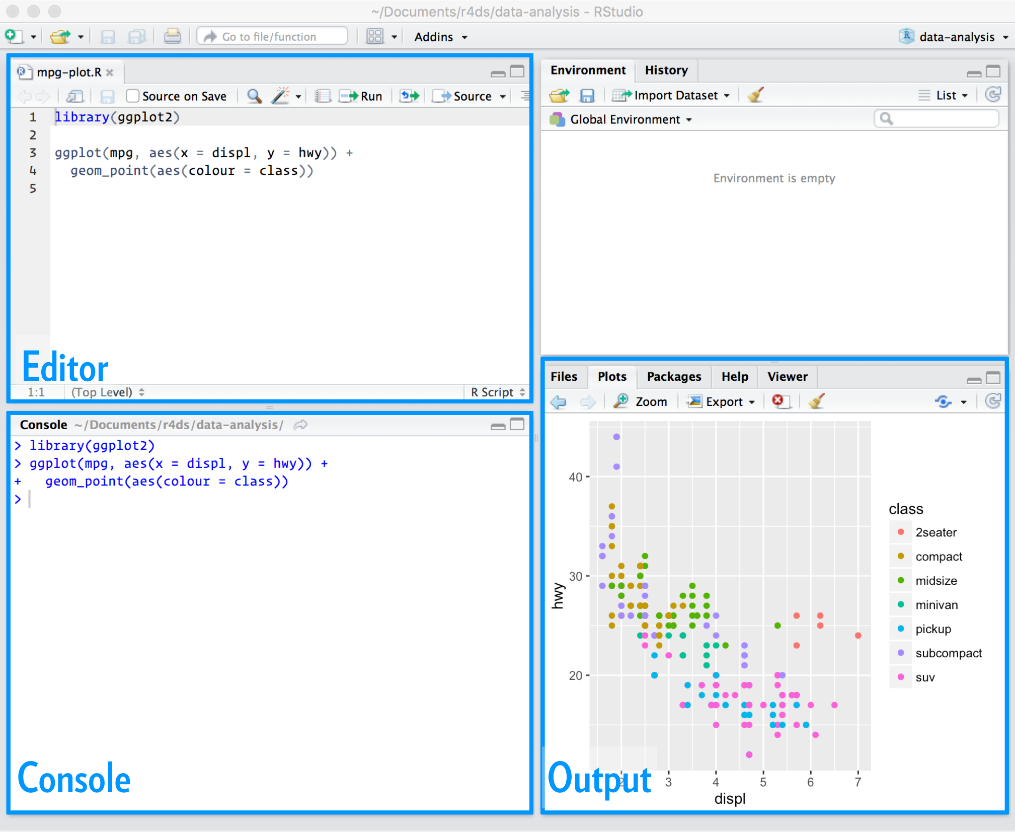
\includegraphics{Figuras/panel.png}

}

\caption{Painés do Rstudio}

\end{figure}%

\begin{itemize}
\tightlist
\item
  Segue uma breve explicação das telas principais do RStudio.
\end{itemize}

\begin{enumerate}
\def\labelenumi{\arabic{enumi}.}
\item
  \textbf{Console:}

  \begin{itemize}
  \tightlist
  \item
    A tela principal onde você digita comandos R e recebe a saída
    imediata.
  \end{itemize}
\item
  \textbf{Script Editor:}

  \begin{itemize}
  \tightlist
  \item
    Onde você escreve e edita seus scripts em R. Os scripts são arquivos
    contendo código R que podem ser executados no console.
  \end{itemize}
\item
  \textbf{Environment/Painel de Ambiente:}

  \begin{itemize}
  \tightlist
  \item
    Exibe informações sobre objetos (variáveis, datasets) em sua sessão
    R atual.
  \end{itemize}
\item
  \textbf{History/Histórico:}

  \begin{itemize}
  \tightlist
  \item
    Mantém um histórico de comandos R previamente executados.
  \end{itemize}
\item
  \textbf{Files/Painel de Arquivos:}

  \begin{itemize}
  \tightlist
  \item
    Mostra os arquivos e diretórios do seu projeto. Facilita a navegação
    e a organização.
  \end{itemize}
\item
  \textbf{Plots/Painel de Gráficos:}

  \begin{itemize}
  \tightlist
  \item
    Exibe visualizações geradas a partir do R.
  \end{itemize}
\item
  \textbf{Packages/Pacotes:}

  \begin{itemize}
  \tightlist
  \item
    Gerencia pacotes R instalados e fornece ferramentas para instalação
    e atualização.
  \end{itemize}
\item
  \textbf{Help/Ajuda:}

  \begin{itemize}
  \tightlist
  \item
    Fornece acesso à documentação e ajuda sobre funções e pacotes R.
  \end{itemize}
\item
  \textbf{Viewer/Visualizador:}

  \begin{itemize}
  \tightlist
  \item
    Exibe visualizações mais complexas, como páginas web, no próprio
    IDE.
  \end{itemize}
\item
  \textbf{Git:}

  \begin{itemize}
  \tightlist
  \item
    Facilita a integração com sistemas de controle de versão Git,
    permitindo o rastreamento de alterações em projetos.
  \end{itemize}
\item
  \textbf{Connections/Conexões:}

  \begin{itemize}
  \tightlist
  \item
    Permite conectar-se a fontes de dados externas
  \end{itemize}
\item
  \textbf{Terminal:}

  \begin{itemize}
  \tightlist
  \item
    Um terminal embutido para execução de comandos do sistema
    operacional.
  \end{itemize}
\end{enumerate}

\subsection{Cheatsheets}\label{cheatsheets}

\begin{itemize}
\item
  As ``cheatsheets'' (folhas de dicas) no RStudio são recursos visuais e
  resumidos que fornecem informações rápidas e úteis sobre tópicos
  específicos relacionados à linguagem de programação R, ao ambiente
  RStudio e a pacotes específicos do R.
\item
  Para acessar as cheatsheets, você pode ir diretamente à
  \href{https://rstudio.com/resources/cheatsheets/}{\ul{página de
  cheatsheets do RStudio}}
\item
  Também pode ser acessada cliclando em Help -\textgreater{} Cheat
  Sheets
\end{itemize}

\section{Caminhos e Diretório de
trabalho}\label{caminhos-e-diretuxf3rio-de-trabalho}

\subsection{Caminhos}\label{caminhos}

\begin{itemize}
\item
  Entende-se por \textbf{caminho} o endereço do arquivo no computador
\item
  Existem duas formas de passarmos o caminho de arquivo: \textbf{caminho
  absoluto} ou \textbf{caminho relativo}
\end{itemize}

\subsection{Caminho Absoluto}\label{caminho-absoluto}

\begin{itemize}
\item
  O \textbf{caminho absoluto} especifica o local exato de um arquivo
  desde a raiz do sistema de arquivo.
\item
  O diretório raiz é o que está no topo da hierarquia do sistema, isso
  significa que outros diretórios estão contidos nele.
\end{itemize}

\begin{figure}[H]

{\centering 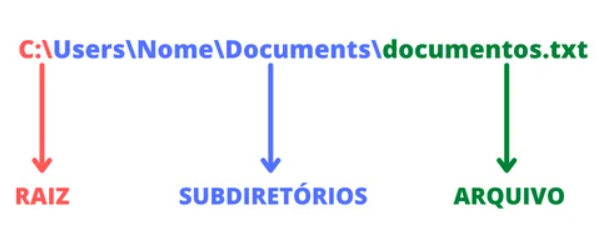
\includegraphics{Figuras/dir_geral.png}

}

\caption{Caminho Absoluto}

\end{figure}%

\begin{itemize}
\tightlist
\item
  \texttt{getwd()} é uma forma abreviada de dizer \emph{get working
  directory} (me diga qual a pasta de trabalho atual).
\end{itemize}

\begin{Shaded}
\begin{Highlighting}[]
\FunctionTok{getwd}\NormalTok{()}
\end{Highlighting}
\end{Shaded}

\begin{verbatim}
[1] "C:/Users/Leonardo_Nascimento/Documents/GitHub/webpage/Cursos/Introducao_R/Cadernos"
\end{verbatim}

\begin{itemize}
\tightlist
\item
  Observe que o local de referência é a pasta ``\emph{Cadernos}'', pois
  este é o caminho absoluto para a pasta onde essa aula foi produzida.
  Vamos voltar para a pasta ``\emph{Introducao\_R}'' utilizando o
  conceito de caminho relativo
\end{itemize}

\subsection{Caminho Relativo}\label{caminho-relativo}

\begin{itemize}
\item
  O \textbf{caminho relativo} é especificado em relação ao diretório de
  trabalho atual ou a outro local de referência. Assim, se você quiser
  acessar alguma base de dados na pasta ``\emph{dados''} partindo da
  pasta''\emph{Cadernos'',} o caminho seria\emph{:}
  \texttt{../dados/base\_de\_dados.formato}.
\item
  Nesse caso, \texttt{../} é o comando para voltar uma pasta dentro do
  caminho e \texttt{./} representa a pasta/diretório atual.
\item
  Caso você queira trocar o local referência da pasta ``\emph{caderno''}
  para a pasta''\emph{Introducao\_R} ``, use o seguinte código:
\end{itemize}

\begin{Shaded}
\begin{Highlighting}[]
\FunctionTok{setwd}\NormalTok{(}\StringTok{".."}\NormalTok{) }\CommentTok{\# trocando local referência ou diretório de trabalho}
\FunctionTok{getwd}\NormalTok{()}
\end{Highlighting}
\end{Shaded}

\begin{verbatim}
[1] "C:/Users/Leonardo_Nascimento/Documents/GitHub/webpage/Cursos/Introducao_R"
\end{verbatim}

\subsection{Diretório de trabalho}\label{diretuxf3rio-de-trabalho}

\begin{itemize}
\item
  Basicamente, diretório de trabalho refere-se a uma pasta específica no
  sistema de arquivos do computador em que um programa está atualmente
  operando ou onde ele procura por arquivos para ler e salvar por
  padrão.
\item
  No contexto do R, o diretório de trabalho é particularmente importante
  porque é o local onde o R procura por arquivos . Isso significa que,
  se você carregar ou salvar um arquivo sem especificar a pasta, o R
  assumirá que o arquivo está no diretório de trabalho.
\item
  É no diretório de trabalho que o R procura os arquivos que você pede
  para carregar e onde ele coloca todos os arquivos que você pede para
  salvar. De forma geral, é o local que está localizada sua análise.
\item
  RStudio mostra seu diretório de trabalho atual na parte superior do
  console:
\end{itemize}

\begin{figure}[H]

{\centering 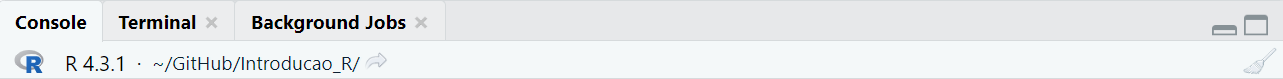
\includegraphics{Figuras/dir.png}

}

\caption{Diretório}

\end{figure}%

\begin{itemize}
\item
  Você também pode visualizar o diretório de trabalho atual usando a
  função \textbf{\texttt{getwd().}}
\item
  Você também pode definir o diretório de trabalho dentro do R
  utilizando a

  função \texttt{setwd("colocar\_o\_caminho").}
\end{itemize}

\subsection{Observações}\label{observauxe7uxf5es}

\begin{itemize}
\item
  Caminhos e diretórios são um pouco complicados porque existem dois
  estilos básicos de caminhos: Mac/Linux e Windows. Existem três
  maneiras principais pelas quais eles diferem

  \begin{enumerate}
  \def\labelenumi{\arabic{enumi}.}
  \item
    Como você separa os componentes do caminho. Mac e Linux usam barras
    (por exemplo~ \texttt{plots/diamonds.pdf}) e o Windows usa barras
    invertidas (por exemplo~
    \texttt{plots\textbackslash{}diamonds.pdf}). R pode funcionar com
    qualquer tipo. Porém, barras invertidas significam algo especial
    para R, e para obter uma única barra invertida no caminho, você
    precisa digitar duas barras invertidas! Recomendo sempre usar o
    estilo Linux/Mac com barras.
  \item
    Ao criar scripts ou projetos em R, é uma boa prática \textbf{usar
    caminhos relativos}, pois isso torna o código mais portátil e
    facilita a colaboração. Além disso, evita problemas quando você
    compartilha seu código com outros ou move seu projeto para um novo
    sistema operacional.
  \item
    A última pequena diferença é o local para onde
    \texttt{\textasciitilde{}}aponta. \texttt{\textasciitilde{}}é um
    atalho conveniente para o seu diretório inicial. No Windows, ele
    aponta para o diretório de documentos. undefined
  \end{enumerate}
\end{itemize}

\subsubsection{Tabela 1: Localização de pastas no
Linux}\label{tabela-1-localizauxe7uxe3o-de-pastas-no-linux}

\begin{longtable}[]{@{}ll@{}}
\toprule\noalign{}
Nome fantasia & Localização real \\
\midrule\noalign{}
\endhead
\bottomrule\noalign{}
\endlastfoot
Pasta pessoal & \texttt{/home/estudante} ou
\texttt{\textasciitilde{}/} \\
Área de trabalho & \texttt{/home/estudante/Desktop} \\
Pendrive & \texttt{/media/RotuloDoPendrive} \\
\end{longtable}

\subsubsection{Tabela 2: Localização de pastas em versão recente do
Windows}\label{tabela-2-localizauxe7uxe3o-de-pastas-em-versuxe3o-recente-do-windows}

\begin{longtable}[]{@{}ll@{}}
\toprule\noalign{}
Nome fantasia & Localização real \\
\midrule\noalign{}
\endhead
\bottomrule\noalign{}
\endlastfoot
Pasta pessoal & \texttt{C:/Users/estudante/Meus\ documentos} ou
\texttt{\textasciitilde{}/} \\
Área de trabalho & \texttt{C:/Users/estudante/Desktop} ou
\texttt{\textasciitilde{}/../Desktop} \\
Pendrive & \texttt{F:/} (ou outra letra) \\
\end{longtable}

\begin{itemize}
\item
  Nesses casos, criar projetos no R é uma prática recomendada e traz
  vários benefícios para a organização, colaboração e reprodutibilidade
  do trabalho
\item
  Crie um diretório onde você possa colocar todos os programas/projetos
  em R
\end{itemize}

\section{Projetos}\label{projetos}

\begin{itemize}
\item
  Projetos no RStudio são uma maneira organizada e estruturada de
  trabalhar em análises de dados e programação em R ou em qualquer
  linguagem de programação suportada pelo RStudio.
\item
  Aqui estão algumas razões pelas quais criar projetos no RStudio é
  importante:

  \begin{enumerate}
  \def\labelenumi{\arabic{enumi}.}
  \item
    \textbf{Organização Estruturada:}

    \begin{itemize}
    \tightlist
    \item
      Projetos fornecem uma estrutura organizada para seus arquivos,
      dados e scripts. Isso facilita a navegação e a localização de
      recursos específicos relacionados ao projeto.
    \end{itemize}
  \item
    \textbf{Reprodutibilidade:}

    \begin{itemize}
    \tightlist
    \item
      Ao criar um projeto, você organiza seu trabalho de forma que seja
      mais fácil reproduzir suas análises. Outros usuários podem
      reproduzir facilmente os resultados, garantindo a
      reprodutibilidade do trabalho.
    \end{itemize}
  \item
    \textbf{Configuração do Diretório de Trabalho:}

    \begin{itemize}
    \tightlist
    \item
      O projeto define automaticamente o diretório de trabalho,
      eliminando a necessidade de definir caminhos relativos em seus
      scripts. Isso reduz erros e torna o código mais portátil.
    \end{itemize}
  \item
    \textbf{Controle de Versão:}

    \begin{itemize}
    \tightlist
    \item
      Projetos podem ser vinculados a sistemas de controle de versão,
      como o Git. Isso facilita o controle de alterações em seus scripts
      e colaboração em equipes.
    \end{itemize}
  \item
    \textbf{Ambiente Isolado:}

    \begin{itemize}
    \tightlist
    \item
      Projetos têm seu próprio ambiente no RStudio. Isso significa que
      as bibliotecas (pacotes) e as configurações específicas do projeto
      não interferem em outros projetos ou em seu ambiente global.
    \end{itemize}
  \end{enumerate}
\item
  A seguir são apresentados alguns passos para criar um projeto no
  RStudio.
\item
  \textbf{Passo 1}: Abra o RStudio

  \begin{itemize}
  \tightlist
  \item
    Inicie o RStudio em seu computador.
  \end{itemize}
\item
  \textbf{Passo 2}: Crie um Novo Projeto

  \begin{itemize}
  \tightlist
  \item
    No canto superior direito do RStudio, clique em ``File'' (Arquivo) e
    selecione ``New Project'' (Novo Projeto).
  \end{itemize}
\end{itemize}

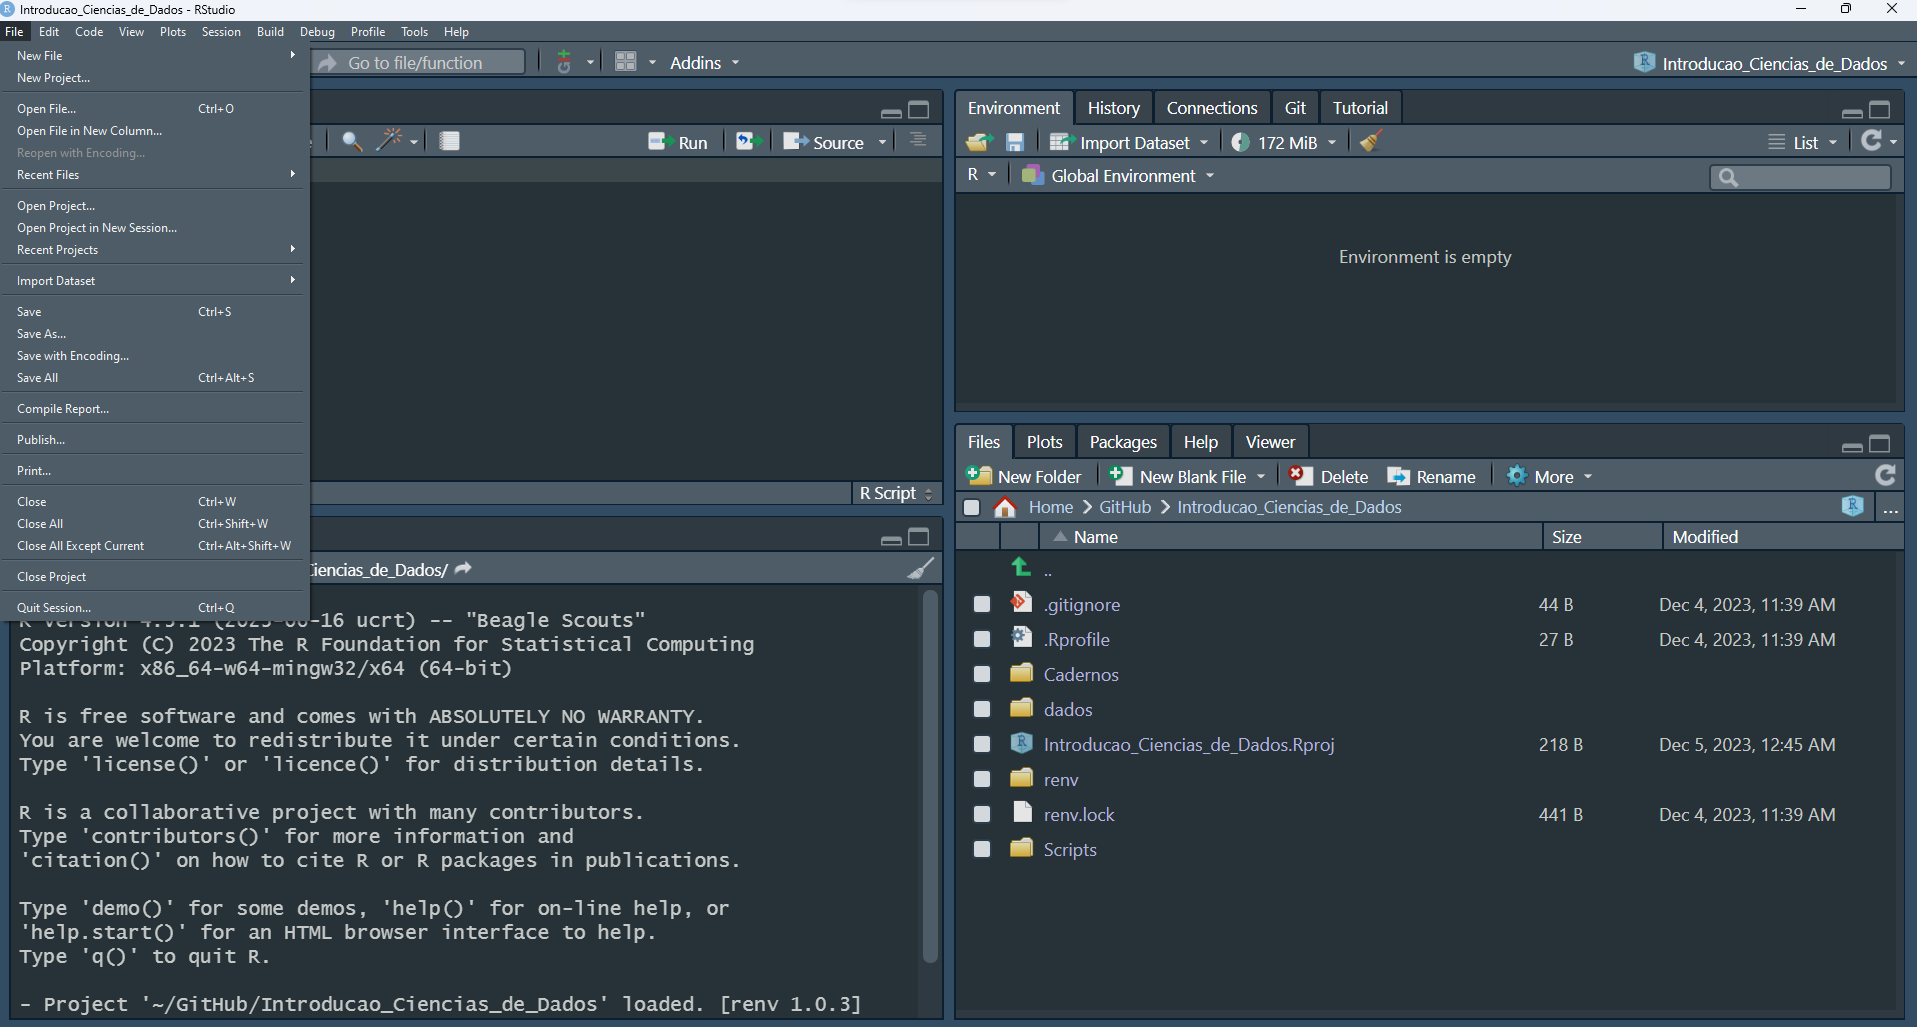
\includegraphics[width=1\textwidth,height=\textheight]{Figuras/proj_1.png}

\begin{itemize}
\item
  \textbf{Passo 3}: Escolha o Tipo de Projeto

  \begin{enumerate}
  \def\labelenumi{\arabic{enumi}.}
  \item
    New Directory (Novo Diretório): Cria um novo diretório para o
    projeto.
  \item
    Existing Directory (Diretório Existente): Usa um diretório existente
    como projeto.
  \end{enumerate}
\end{itemize}

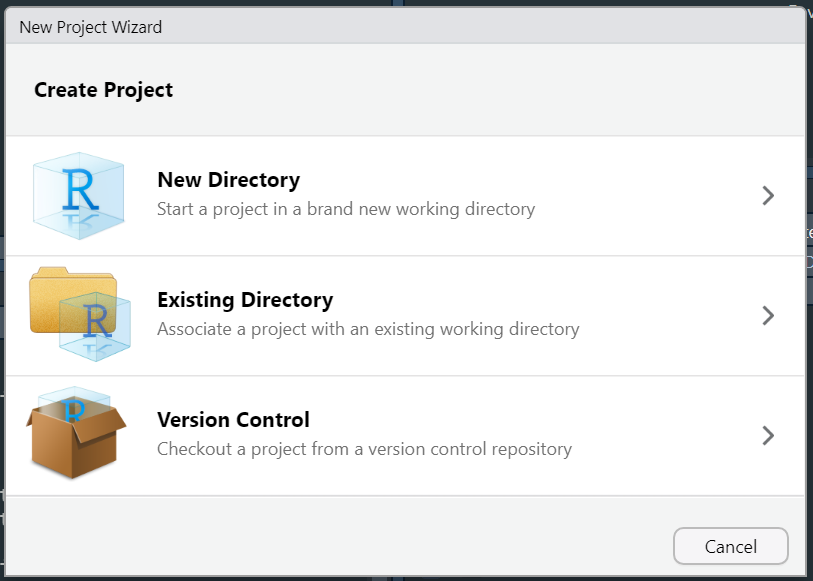
\includegraphics[width=5.20833in,height=\textheight]{Figuras/proj_2.png}

\begin{itemize}
\item
  \textbf{Passo 4}: Escolha um Modelo

  \begin{itemize}
  \tightlist
  \item
    Você pode escolher um modelo específico se estiver disponível. Caso
    contrário, escolha ``New Project'' (Novo Projeto).
  \end{itemize}
\end{itemize}

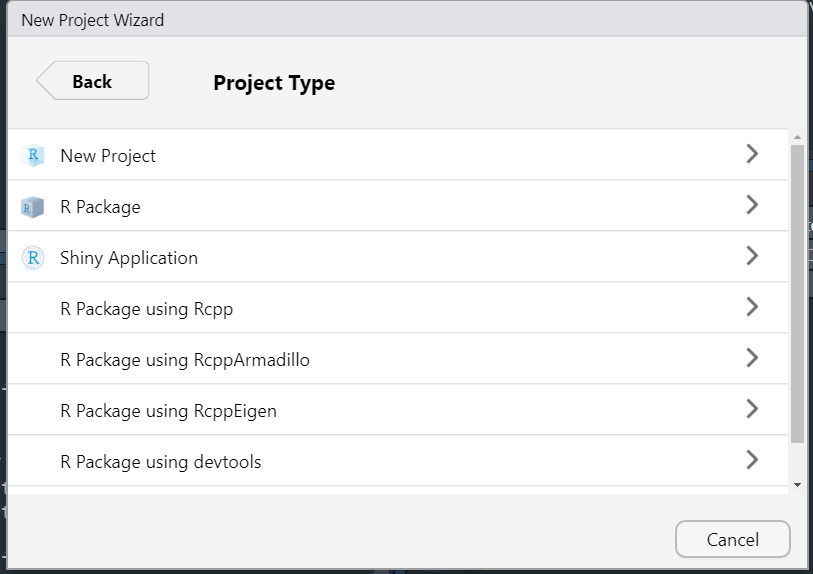
\includegraphics[width=5.20833in,height=\textheight]{Figuras/proj_3.png}

\begin{itemize}
\item
  \textbf{Passo 5}: Nomeie e Localize o Projeto

  \begin{itemize}
  \tightlist
  \item
    Dê um nome ao seu projeto e escolha o local onde o diretório do
    projeto será armazenado.
  \end{itemize}
\end{itemize}

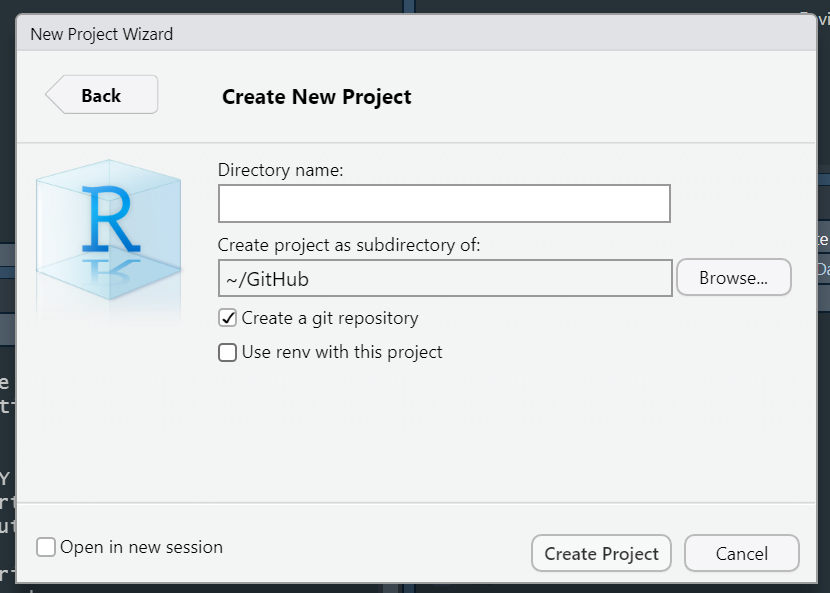
\includegraphics[width=132mm,height=\textheight]{Figuras/proj_4.png}

\begin{itemize}
\item
  \textbf{Passo 6}: Clique em ``Create Project''

  \begin{itemize}
  \tightlist
  \item
    Clique em ``Create Project'' (Criar Projeto) para finalizar a
    criação do projeto.
  \end{itemize}
\item
  Após criar o projeto, você verá a estrutura do diretório do projeto no
  painel inferior direito do RStudio.
\item
  Organize seus Arquivos. Dentro do diretório do projeto, você pode
  criar subdiretórios (por exemplo, ``data'', ``scripts'', ``reports'')
  para organizar seus arquivos.
\item
  Tudo o que você precisa está em um só lugar e bem separado de todos os
  outros projetos nos quais você está trabalhando.
\end{itemize}

\subsubsection{Configuração}\label{configurauxe7uxe3o}

\begin{itemize}
\item
  Basicamente, podemos definir uma \textbf{pesquisa reproduzível} como
  uma pesquisa que documenta todas as etapas entre os dados brutos e os
  resultados de uma forma que possa ser verificada.
\item
  Isso envolve escrever scripts que realizem algumas análises do início
  ao fim de forma completa e transparente, de maneira que produza o
  mesmo resultado para pessoas diferentes usando o mesmo software em
  computadores diferentes.
\item
  Nesse caso, é \textbf{recomendado} realizar dois ajustes na
  configuração do RStudio para maximizar a reprodutibilidade. Será
  desabilitado \texttt{.RData\ e\ .Rhistory.}
\item
  O primeiro armazena todos os objetos gerados durante uma sessão R,
  enquanto o segundo mantém uma lista dos comandos mais recentemente
  executados.
\item
  Ao reabrir o RStudio, o conteúdo desses arquivos é carregado no
  ambiente de trabalho atual, proporcionando a sensação de continuidade.
\item
  Selecione \textbf{Tools \textgreater{} Global Options\ldots{}} na aba
  de ferramentas do RStudio e então ajustar as configurações.
\item
  A página de configurações gerais deve apresentar semelhanças com a
  imagem a seguir:
\end{itemize}

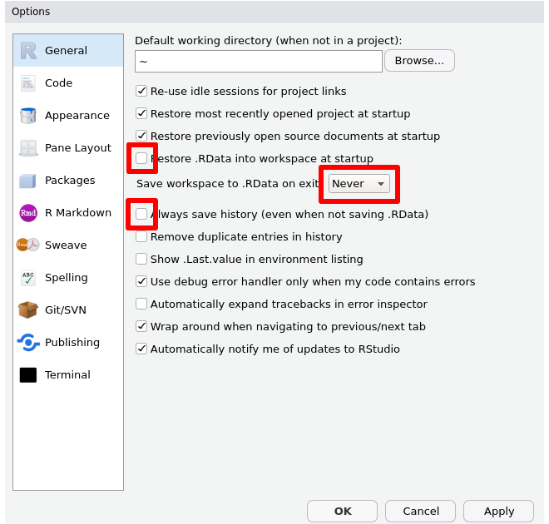
\includegraphics{Figuras/options.png}

\section{PositCloud}\label{positcloud}

\begin{itemize}
\item
  Plataforma online que utiliza o RStudio para auxiliar na análise de
  dados ou outras finalidades.
\item
  Para acessá-la, clique
  \href{https://login.posit.cloud/login?redirect=\%2F}{aqui}.
\item
  Para criar um projeto:
\end{itemize}

\includegraphics[width=1\textwidth,height=\textheight]{Figuras/posit.gif}

\section{Git e GitHub}\label{git-e-github}

\begin{itemize}
\item
  Git é um sistema de controle de versão que permite rastrear as
  alterações no código durante o desenvolvimento de uma
  análise/software.
\item
  Git é usado para gerenciar projetos de análise/software, controlar as
  versões do código e facilitar o trabalho colaborativo entre
  desenvolvedores.
\item
  Cada cópia do repositório Git contém todo o histórico de revisões.
\item
  Permite a criação de ramificações independentes para o desenvolvimento
  de novos recursos e a fusão posterior dessas ramificações.
\item
  O Git também pode se conectar a um serviço de hospedagem e armazenar
  todas as versões de um código fora do seu computador; o mais utilizado
  atualmente se chama GitHub. Uma alternativa é o GitLab.
\item
  GitHub oferece funcionalidades adicionais, como controle de acesso,
  rastreamento de problemas, integração contínua e colaboração
  eficiente.
\item
  Desenvolvedores usam o GitHub para compartilhar código, colaborar em
  projetos e contribuir para repositórios de código aberto.
\end{itemize}

\begin{figure}[H]

{\centering 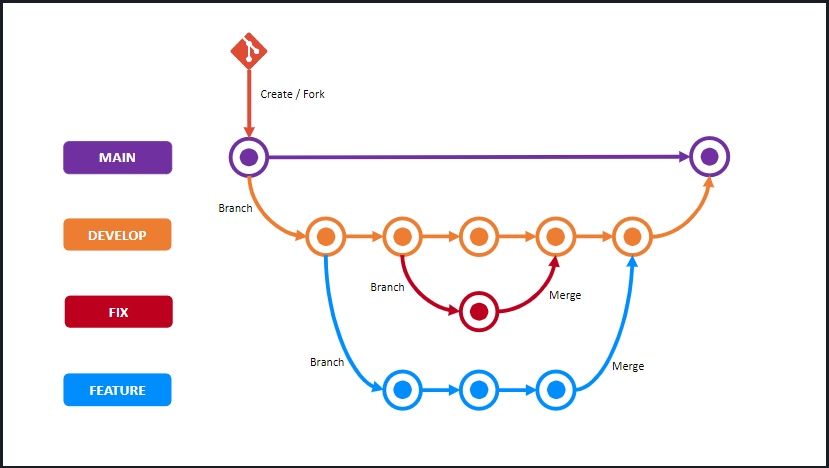
\includegraphics[width=1\textwidth,height=\textheight]{Figuras/git_ideia.png}

}

\caption{Ideia geral do funcionamento do Git}

\end{figure}%

\begin{itemize}
\item
  Na prática, a utilização do Git e do GitHub tem dois principais
  benefícios:

  \begin{itemize}
  \item
    Livrar-se da necessidade de controlar versões com arquivos como
    \texttt{analise.R}, \texttt{analise\_v2.R}, \texttt{analise\_v3.R},
    \texttt{analise\_final.R}, \texttt{analise\_final\_final.R},
    \texttt{analise\_final\_revisada.R}
  \item
    Eliminar a preocupação de perder seus projetos devido a falhas no
    seu computador.
  \end{itemize}
\end{itemize}

\section{Pacotes}\label{pacotes}

\begin{itemize}
\item
  É muito provável que alguém já tenha resolvido o problema em que você
  está trabalhando, e você pode se beneficiar do trabalho deles baixando
  o pacote correspondente.
\item
  Um pacote reúne código, dados e documentação, proporcionando um método
  fácil de compartilhamento com outros usuários.
\end{itemize}

\begin{center}
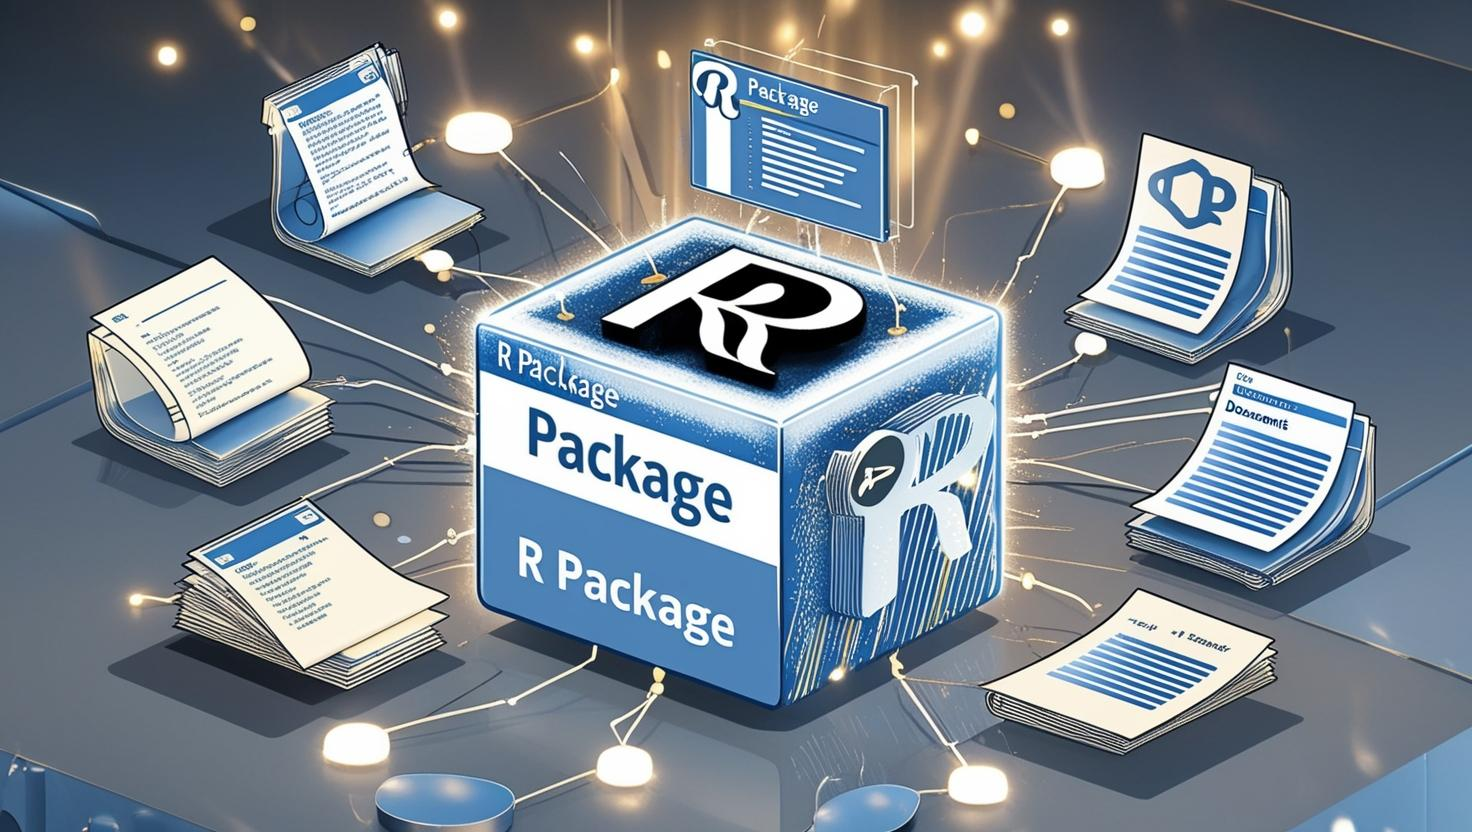
\includegraphics[width=5.19792in,height=\textheight]{Figuras/rpackage.jpg}
\end{center}

\subsection{Instalação}\label{instalauxe7uxe3o}

\begin{itemize}
\item
  O R é construído como um conjunto de bibliotecas/pacotes voltadas para
  diferentes aplicações;
\item
  Todos esses pacotes (com a respectiva documentação) podem ser
  facilmente baixados e instalados a partir do repositório CRAN.
\item
  No entanto, muitas vezes, durante a programação, é necessário um
  pacote adicional para o nosso projeto. O RStudio permite baixar e
  instalá-lo através da função
  \texttt{install.packages("nome\_do\_pacote")};
\item
  Por exemplo, para instalar o pacote ggplot2 (Wickham 2016):
  \texttt{install.packages("ggplot2")}. Dessa forma, o pacote ggplot2 e
  os dependentes são automaticamente instalados;
\item
  Para atualizar os pacotes: \textbf{Tools \textgreater{} Check for
  Package Updates\ldots{}}
\item
  Para instalar pacotes do GitHub {[}@{]}:
  \texttt{devtools::install\_github("username/packagename")} . Esse
  comando irá instalar o pacote que está na página
  \texttt{github.com/username/packagename}
\end{itemize}

\subsection{Carregar}\label{carregar}

\begin{itemize}
\item
  Após instalado, o pacote é carregado na atual sessão através do
  comando \texttt{library(ggplot2)} ;
\item
  Outra forma é utilizar: \texttt{ggplot2::nome\_do\_comando}. Nesse
  caso, não precisa carregar o pacote na sessão
\end{itemize}

\section{Solicitando ajuda}\label{solicitando-ajuda}

\begin{Shaded}
\begin{Highlighting}[]
\CommentTok{\# Ver todos os pacotes instalados}
\FunctionTok{library}\NormalTok{()}

\CommentTok{\# Ver pacotes atualmente carregados}
\FunctionTok{search}\NormalTok{()}

\CommentTok{\# Fornece detalhes sobre o conteúdo de um pacote}
\FunctionTok{help}\NormalTok{(}\AttributeTok{package =} \StringTok{"nome\_do\_pacote"}\NormalTok{)}

\CommentTok{\# Fornecer detalhes sobre a base de dados "diamonds" que está dentro do pacote "ggplot2"}

\FunctionTok{help}\NormalTok{(diamonds, }\AttributeTok{package=}\StringTok{"ggplot2"}\NormalTok{)}

\CommentTok{\# Fornecer detalhes sobre o uso da função "mean" que está dentro do pacote base}

\FunctionTok{help}\NormalTok{(mean)}
\NormalTok{?mean}

\CommentTok{\# Listar as vinhetas/tutorias disponíveis para um pacote específico}
\FunctionTok{vignette}\NormalTok{(}\AttributeTok{package =} \StringTok{"nome\_do\_pacote"}\NormalTok{)}

\CommentTok{\# Visualizar uma vinheta específica}
\FunctionTok{vignette}\NormalTok{(}\StringTok{"nome\_da\_vinheta"}\NormalTok{)}

\CommentTok{\# Visualizar todas as vinhetas disponíveis no seu computador}
\FunctionTok{vignette}\NormalTok{()}
\end{Highlighting}
\end{Shaded}

\section{Fluxo de Trabalho}\label{fluxo-de-trabalho}

\begin{itemize}
\tightlist
\item
  Aqui será apresentado um fluxo de trabalho básico que pode
  incrementado no decorrer do curso.
\end{itemize}

\begin{enumerate}
\def\labelenumi{\arabic{enumi}.}
\item
  \textbf{Organize o Projeto:}

  \begin{itemize}
  \item
    Mantenha um diretório de projeto bem estruturado.
  \item
    Use subdiretórios para dados brutos, scripts, figuras e relatórios.
  \end{itemize}
\item
  \textbf{Documente Seu Código:}

  \begin{itemize}
  \item
    Adicione comentários claros e informativos ao seu código.
  \item
    Use R Markdown ou Notebooks R para incorporar narrativa com o
    código.
  \end{itemize}
\item
  \textbf{Versione Seu Código:}

  \begin{itemize}
  \item
    Use um sistema de controle de versão como o Git para controlar as
    mudanças no seu código.
  \item
    Inclua um arquivo \textbf{\texttt{.gitignore}} para evitar a
    inclusão de arquivos desnecessários no repositório.
  \item
    Em \href{https://semver.org/lang/pt-BR/}{SemVer} (\emph{Semantic
    Versioning}) apresenta o padrão de versionamentos. Irei apresentar
    na seção de Pacotes.
  \end{itemize}
\item
  \textbf{Compartilhe Seu Código e Dados:}

  \begin{itemize}
  \tightlist
  \item
    Disponibilize seu código e dados em um repositório público (por
    exemplo, GitHub) ou em um formato acessível.
  \end{itemize}
\end{enumerate}

\section{Escrevendo o código}\label{escrevendo-o-cuxf3digo}

\begin{itemize}
\item
  Ao escrever código, é muito importante ser claro e seguir uma
  estrutura racional. Normalmente, nosso código será depurado, lido,
  usado ou modificado por outras pessoas, portanto, deve ser muito claro
\item
  Uma das práticas recomendadas que mais ajudam na clareza são os
  comentários no código. Eles são frases em linguagem natural precedidas
  por um símbolo de hash \texttt{\#} ou \texttt{\#\textquotesingle{}.}
\item
  Os comentários não são lidos durante a execução do código e servem
  para expressar ideias adicionais que ajudam outras pessoas a
  entenderem o que programamos.
\item
  É possível pegar qualquer \textbf{script R} e compilá-lo em um
  relatório que inclua comentários, código-fonte e saída do script.
\item
  Os relatórios podem ser gerados em diversos formatos, como
  \textbf{HTML, PDF, MS Word e Markdown}.
\item
  Para compilar um relatório \textbf{a partir de um script R}, basta
  passá-lo para a função \texttt{render()}. Por exemplo:
  \texttt{rmarkdown::render("meu\_script.R",pdf\_document)} ou usar o
  comando \emph{Compile Report} command (Ctrl+Shift+K) após a instalação
  do pacote \texttt{rmarkdown} .
\item
  Para realizar os comentários dentro do script R algumas dicas básicas
  são:
\end{itemize}

\begin{Shaded}
\begin{Highlighting}[]
\CommentTok{\#\textquotesingle{} {-}{-}{-}}
\CommentTok{\#\textquotesingle{} title: "Aula 1"}
\CommentTok{\#\textquotesingle{} author: "Leonardo"}
\CommentTok{\#\textquotesingle{} date: "17/03/2025"}

\CommentTok{\#\textquotesingle{} {-}{-}{-}}

\CommentTok{\#\textquotesingle{} Use \#\textquotesingle{} para escrever um texto }
\CommentTok{\#\textquotesingle{} }
\CommentTok{\#\textquotesingle{} Use \# para escrever um texto dentro do código}
\CommentTok{\#\textquotesingle{} }
\CommentTok{\#\textquotesingle{} Pode{-}se criar seções e subseções no código. Selecione Ctrl+Shift+o para identificá{-}las}
  
\CommentTok{\# Seção {-}{-}{-}{-}{-}{-}{-}{-}{-}{-}{-}{-}{-}{-}{-}{-}{-}{-}{-}{-}{-}{-}{-}{-}{-}{-}{-}{-}{-}{-}{-}{-}{-}{-}{-}{-}{-}{-}{-} (Ctrl+Shift+r para criar a seção)}

\CommentTok{\#\textquotesingle{} Realizando a soma de dois números }
\DecValTok{2}\SpecialCharTok{+}\DecValTok{2} \CommentTok{\# o símbolo "+" representa a soma (comentando no código)}

\DocumentationTok{\#\# Subseção {-}{-}{-}{-}{-}{-}{-}{-}}

\CommentTok{\# código}

\DocumentationTok{\#\#\# Subseção da Subseção {-}{-}{-}{-}{-}{-}{-}{-}{-}{-}{-}{-}}
\CommentTok{\# mais código}

\CommentTok{\#\textquotesingle{} Use \# para comentar uma parte do código }
\CommentTok{\#\textquotesingle{} }
\CommentTok{\#\textquotesingle{} Selecione várias linhas de código e use Ctrl+Shift+c para comentar as linhas}
\CommentTok{\#\textquotesingle{} }
\CommentTok{\#\textquotesingle{} Use \#+ para adicionar configurações }
\CommentTok{\#+ fig.width=5, fig.height=5}

\NormalTok{x }\OtherTok{=} \DecValTok{1}\SpecialCharTok{:}\DecValTok{10}\NormalTok{ ; y }\OtherTok{=} \DecValTok{2}\SpecialCharTok{*}\NormalTok{x}
\FunctionTok{plot}\NormalTok{(x,y)}

\CommentTok{\#\textquotesingle{} Escreva expressões matemáticas: $\textbackslash{}bar\{X\}=\textbackslash{}frac\{\textbackslash{}sum\_\{i=1\}\^{}\{n\}x\_i\}\{n\}$}
\CommentTok{\#\textquotesingle{} }
\CommentTok{\#\textquotesingle{} A média de x é \textasciigrave{}r mean(x)\textasciigrave{}}
\end{Highlighting}
\end{Shaded}

\begin{itemize}
\tightlist
\item
  O código acima gera o seguinte documento html:
\end{itemize}

\begin{center}
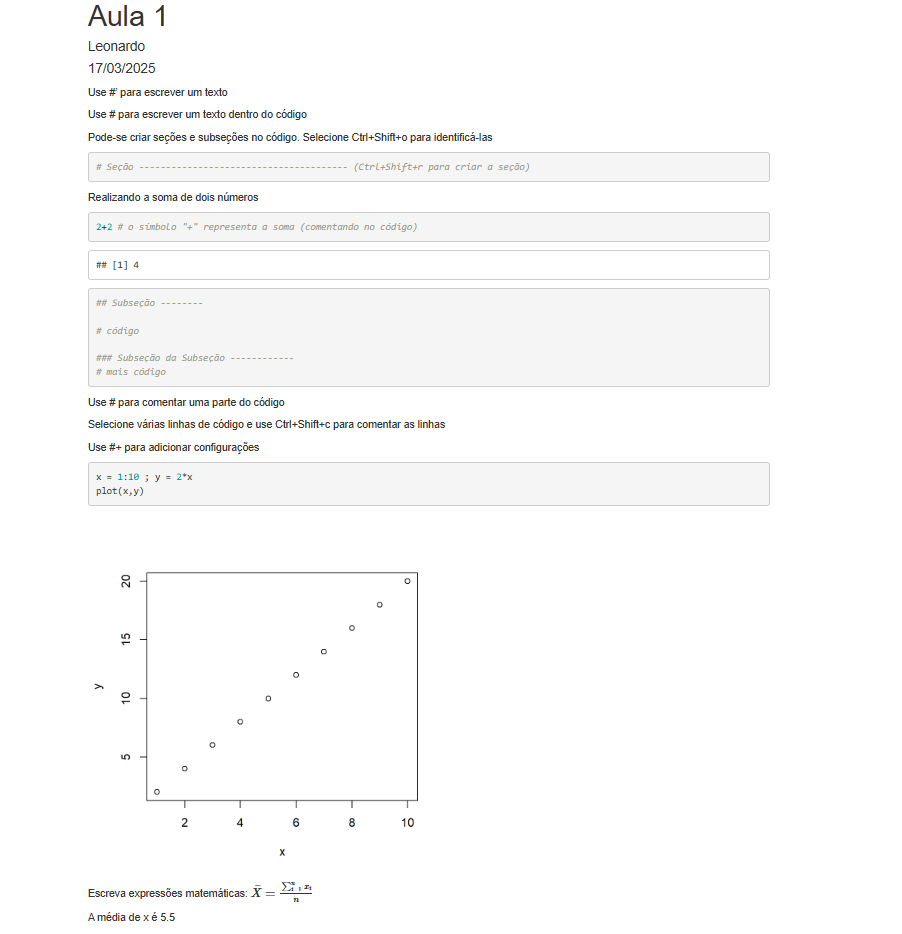
\includegraphics{Figuras/doc.png}
\end{center}

\begin{itemize}
\item
  Um dos melhores ambientes para desenvolvimento de código é um arquivo
  RMarkdown. Recentemente foi criado o Quarto com o mesmo objetivo. Para
  mais detalhes sobre documentação dinâmica, pesquisar sobre os pacotes
  \texttt{rmarkdown} e o aplicatico \texttt{Quarto} para R.\\
\item
  Para criar um arquivo Rmarkdown, basta clicar em File \textgreater{}
  New File \textgreater{} R Markdown

  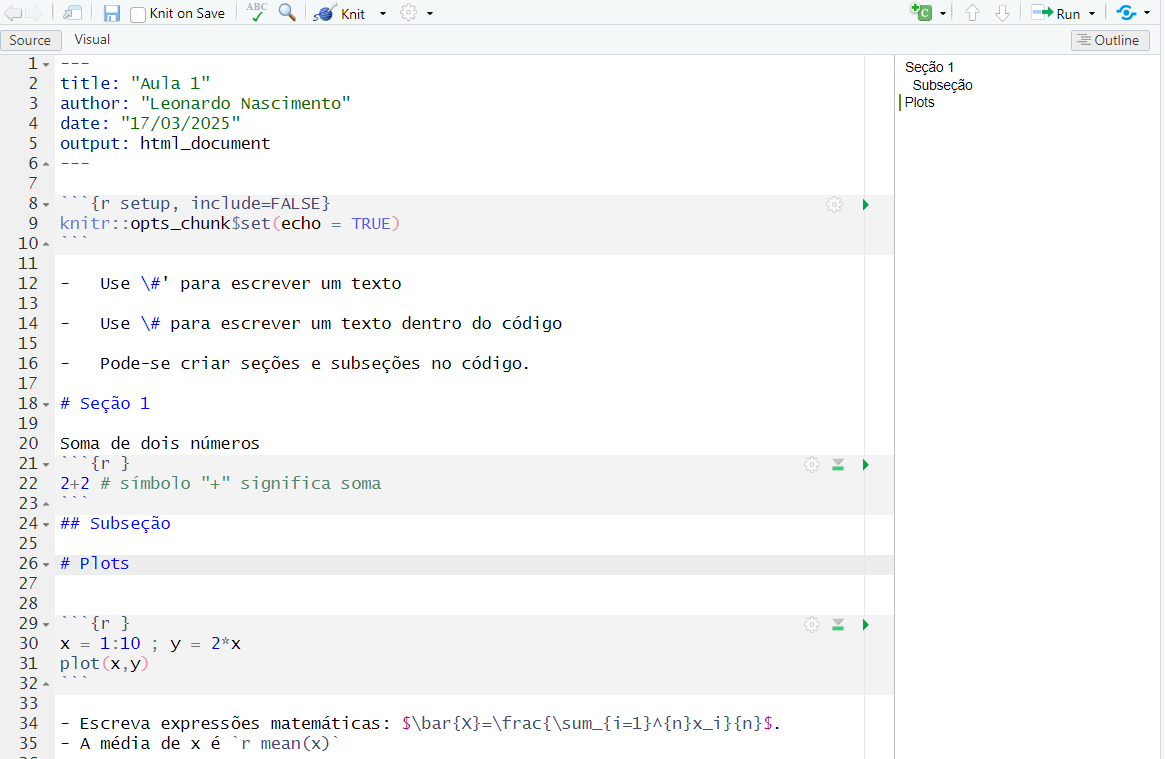
\includegraphics[width=6.125in,height=\textheight]{Figuras/rmd.png}
\end{itemize}

\section{R e Ciência de Dados}\label{r-e-ciuxeancia-de-dados}

\begin{itemize}
\item
  Ciência de dados é um conjunto de ferramentas que permite o
  pesquisador transformar dados brutos em compreensão,~\emph{insights}~e
  conhecimento.
\item
  Aprender as ferramentas mais importantes em R, permitirão que o
  pesquisador realize ciência de dados de forma eficiente e reprodutível
\item
  A ciência de dados é um campo vasto e por isso vamos seguir as
  seguintes etapas:
\end{itemize}

\begin{center}
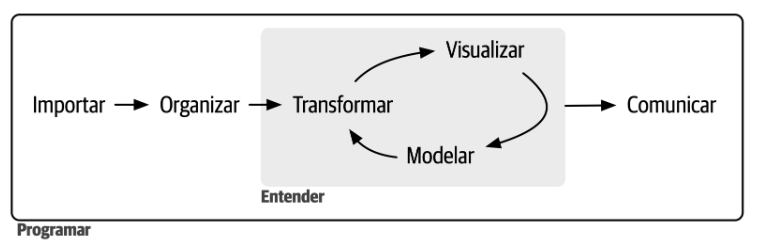
\includegraphics{Figuras/fases_da_CD.png}
\end{center}

\begin{enumerate}
\def\labelenumi{\arabic{enumi}.}
\item
  O pesquisador começa com a importação e organização dos dados.
\item
  Em seguida, entende seus dados por meio de um ciclo iterativo de
  transformação, visualização e modelagem.
\item
  Por fim, finaliza o ciclo comunicando seus resultados para outras
  pessoas.
\end{enumerate}

\begin{itemize}
\item
  Todas essas etapas são realizadas utilizando a linguagem de
  programação em R integradas com outras linguagens
\item
  Algumas referências para o curso: Irizarry (2019),Boehmke (2016),
  Wickham, Grolemund, et al. (2017), Zamora Saiz et al. (2020) e Wickham
  (2019)
\end{itemize}

\section{Atividades}\label{atividades}

\begin{itemize}
\item
  Crie uma conta no \href{https://github.com/}{\ul{Github}}
\item
  Crie um projeto
\end{itemize}

\phantomsection\label{refs}
\begin{CSLReferences}{1}{0}
\bibitem[\citeproctext]{ref-boehmke2016data}
Boehmke, Bradley C. 2016. \emph{Data wrangling with R}. Springer.

\bibitem[\citeproctext]{ref-irizarry2019introduction}
Irizarry, Rafael A. 2019. \emph{Introduction to data science: Data
analysis and prediction algorithms with R}. Chapman; Hall/CRC.

\bibitem[\citeproctext]{ref-ggplot2}
Wickham, Hadley. 2016. {«ggplot2: Elegant Graphics for Data Analysis»}.
\url{https://ggplot2.tidyverse.org}.

\bibitem[\citeproctext]{ref-wickham2019advanced}
---------. 2019. \emph{Advanced r}. chapman; hall/CRC.

\bibitem[\citeproctext]{ref-wickham2017r}
Wickham, Hadley, Garrett Grolemund, et al. 2017. \emph{R for data
science}. Vol. 2. O'Reilly Sebastopol, CA.

\bibitem[\citeproctext]{ref-ZamoraSaiz2020}
Zamora Saiz, Alfonso, Carlos Quesada González, Lluís Hurtado Gil, e
Diego Mondéjar Ruiz. 2020. \emph{An Introduction to Data Analysis in R:
Hands-on Coding, Data Mining, Visualization and Statistics from
Scratch}. Springer International Publishing.

\end{CSLReferences}



\end{document}
